\documentclass[10pt,a4paper,italian]{article}
\usepackage[latin1]{inputenc}
\usepackage{babel}
\usepackage{color}
\usepackage{amssymb}
\usepackage{amsmath}
\usepackage{epsfig}
\usepackage{tabularx}
\usepackage{multirow}
\usepackage{subfigure}
\usepackage{verbatim}
\usepackage{babel}
\usepackage{fancyhdr}
\usepackage{listings}
\usepackage{../common/espacs}

\makeatother

\title{Esercitazione 3}
\date{20/10/2011}

\setlength{\textwidth}{100ex}
\setlength{\oddsidemargin}{0ex}

\pagestyle{fancy}
\headheight 35pt

\rhead{\copyright~Copyright 2006-2011}

\begin{document}
\lstset{language=[ISO]C++}
\maketitle

The solution to the exercise session 2 gives an implementation of different
algorithms to perform the search of a zero of a function $ f \in C^{1} \left(a,
b \right) $ that vanishes at $ \alpha \in \openint{a}{b} $. The code is
organized i na procedural way.

\subsection*{Exercise 1}

Build the connection matrix $B\in \mathbb{R}^{5 \times 5}$ relative to the web
made of the 5 pages, as illustrated in Fig.~\ref{fig:web}.

\begin{figure}
\centering
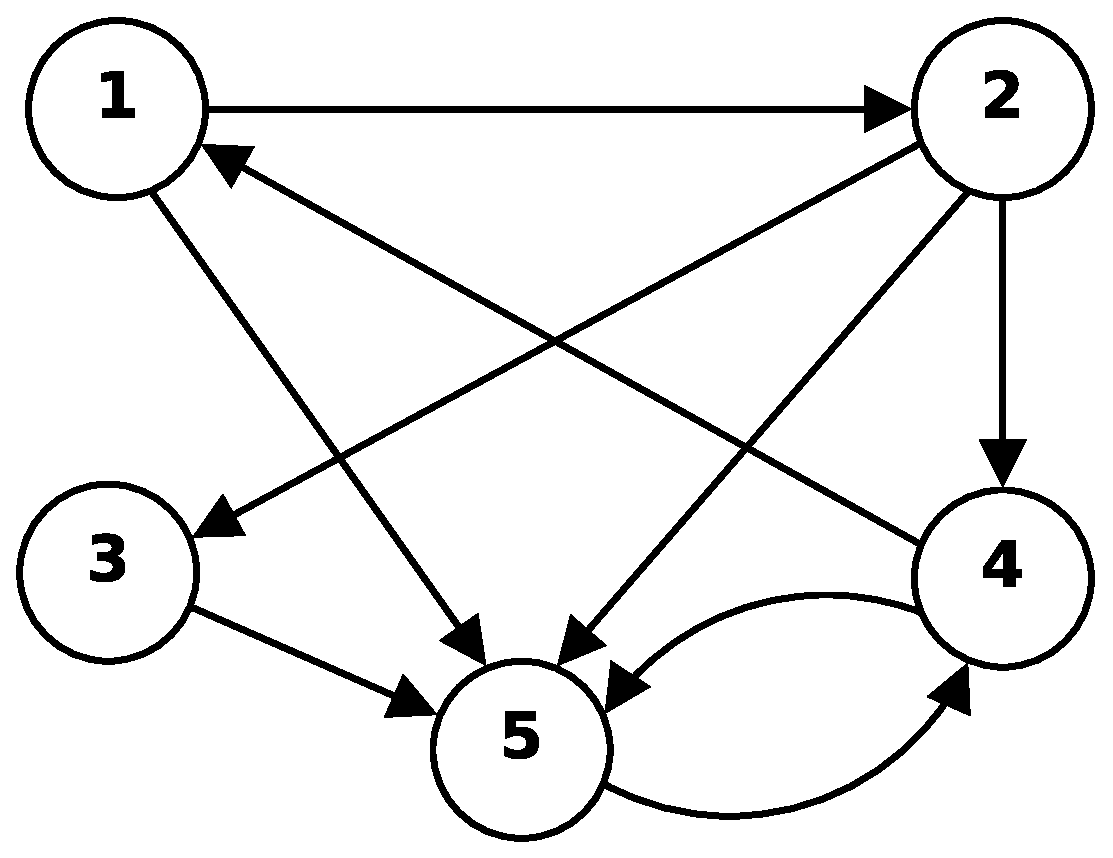
\includegraphics[width=0.5\textwidth]{fig/web}
\caption{Scheme for a 5 pages web. Every circle is a page, every arrow is a
link}
\label{fig:web}
\end{figure}

using the \texttt{Eigen} library, write down a class that computes the maximum
eigenvalue (that is 1) and the corresponding eigenvector, that is the
\emph{pagerank}. Implement also \cpp{operator<<} to see the data inside the
class on the screen.

\subsection*{Soluzione es. 1}

La soluzione dell'esercizio \`e riportata nel seguente listato:
%
\lstset{basicstyle=\scriptsize\sf}
    \lstinputlisting{./es/1/all_in_one/bn-allinone.cpp}
\lstset{basicstyle=\sf}

Si noti, innanzitutto, che \`e stato definito un tipo utente
\cpp{real}. Qualora si volesse modificare la precisione
con cui si effettuano i calcoli, sarebbe sufficiente cambiare solo la
linea contenente la definizione del tipo \cpp{real}. La modifica si
propagherebbe in modo coerente in tutto il codice.

Per rendere l'implementazione dei metodi di ricerca indipendente dalla
funzione considerata si \`e adottata la tecnica dei \emph{puntatori a
funzione}. L'istruzione:
\begin{lstlisting}
typedef real (*fctptr)(real);
\end{lstlisting}
definisce il tipo \cpp{fctptr} come un puntatore a funzioni che
ricevono un argomento di tipo \cpp{real} e restituiscono un valore di
tipo \cpp{real}.

L'arresto dei metodi iterativi per la ricerca degli zeri di una
funzione pu\`o avvenire in base a diversi criteri. Per funzioni che
abbiano derivata prima vicina a $1$ in modulo in corrispondenza dello
zero cercato un efficiente metodo d'arresto \`e basato sul controllo
del \emph{residuo}. In tal caso si considera raggiunta la convergenza
alla prima iterazione $k$ in cui
$\module{\function{f}{x\iter{k}}}<\cpp{tol}$. Un metodo alternativo
basato sul controllo dell'\emph{incremento} risulta, per contro,
efficiente qualora si utilizzino delle iterazioni di punto fisso e la
funzione di iterazione $\function{\phi}{\cdot}$ abbia derivata prima
lontana da $1$ in modulo in corrispondenza dello zero cercato. Tale
criterio prevede l'arresto alla prima iterazione $k$ per cui si abbia
$\module{x\iter{k+1} - x\iter{k}}<\cpp{tol}$. Nel caso del metodo di
Netwon, in cui, per definizione, $\function{\phi'}{\alpha} = 0$, il
controllo dell'incremento fornisce un bilanciamento
ottimale. Nell'implementazione si \`e tenuto conto della
molteplicit\`a dei criteri d'arresto definendo un tipo enumerativo
\cpp{checkT} e dotando ogni metodo di una propriet\`a \cpp{M\_check}
di tipo \cpp{checkT} che specificasse il metodo da utilizzare.

Compilando il codice con i comandi
\begin{verbatim}
    g++ -o bn-allinone bn-allinone.cpp -Wall
\end{verbatim}
Ed eseguendolo, otteniamo
\begin{verbatim}
0.707107        27
0.707107        7
0.707107        14 1
\end{verbatim}


\bibliographystyle{siam}
\bibliography{../common/bibliography}

\end{document}
